%%%%%%%%%%%%%%%%%%%%%%%%%
\section{Use Cases} \label{useCases}
%%%%%%%%%%%%%%%%%%%%%%%%%
In this chapter some of the possible actions that can be performed into \applicationName\ are presented. The aim of this chapter is to provide a practical introduction to \applicationName, through different use cases.
\subsection{Access information}
The first use case presented introduces the available option to access building models data.\\
An InfoBox is shown, whenever a building is selected through a click of the mouse or a tap on the screen of a smartphone. Figure \ref{subfig:infoBox} and Figure \ref{subfig:infoBox_city} shows how these information are given to the user.\\
\begin{figure} [h]
\centering
	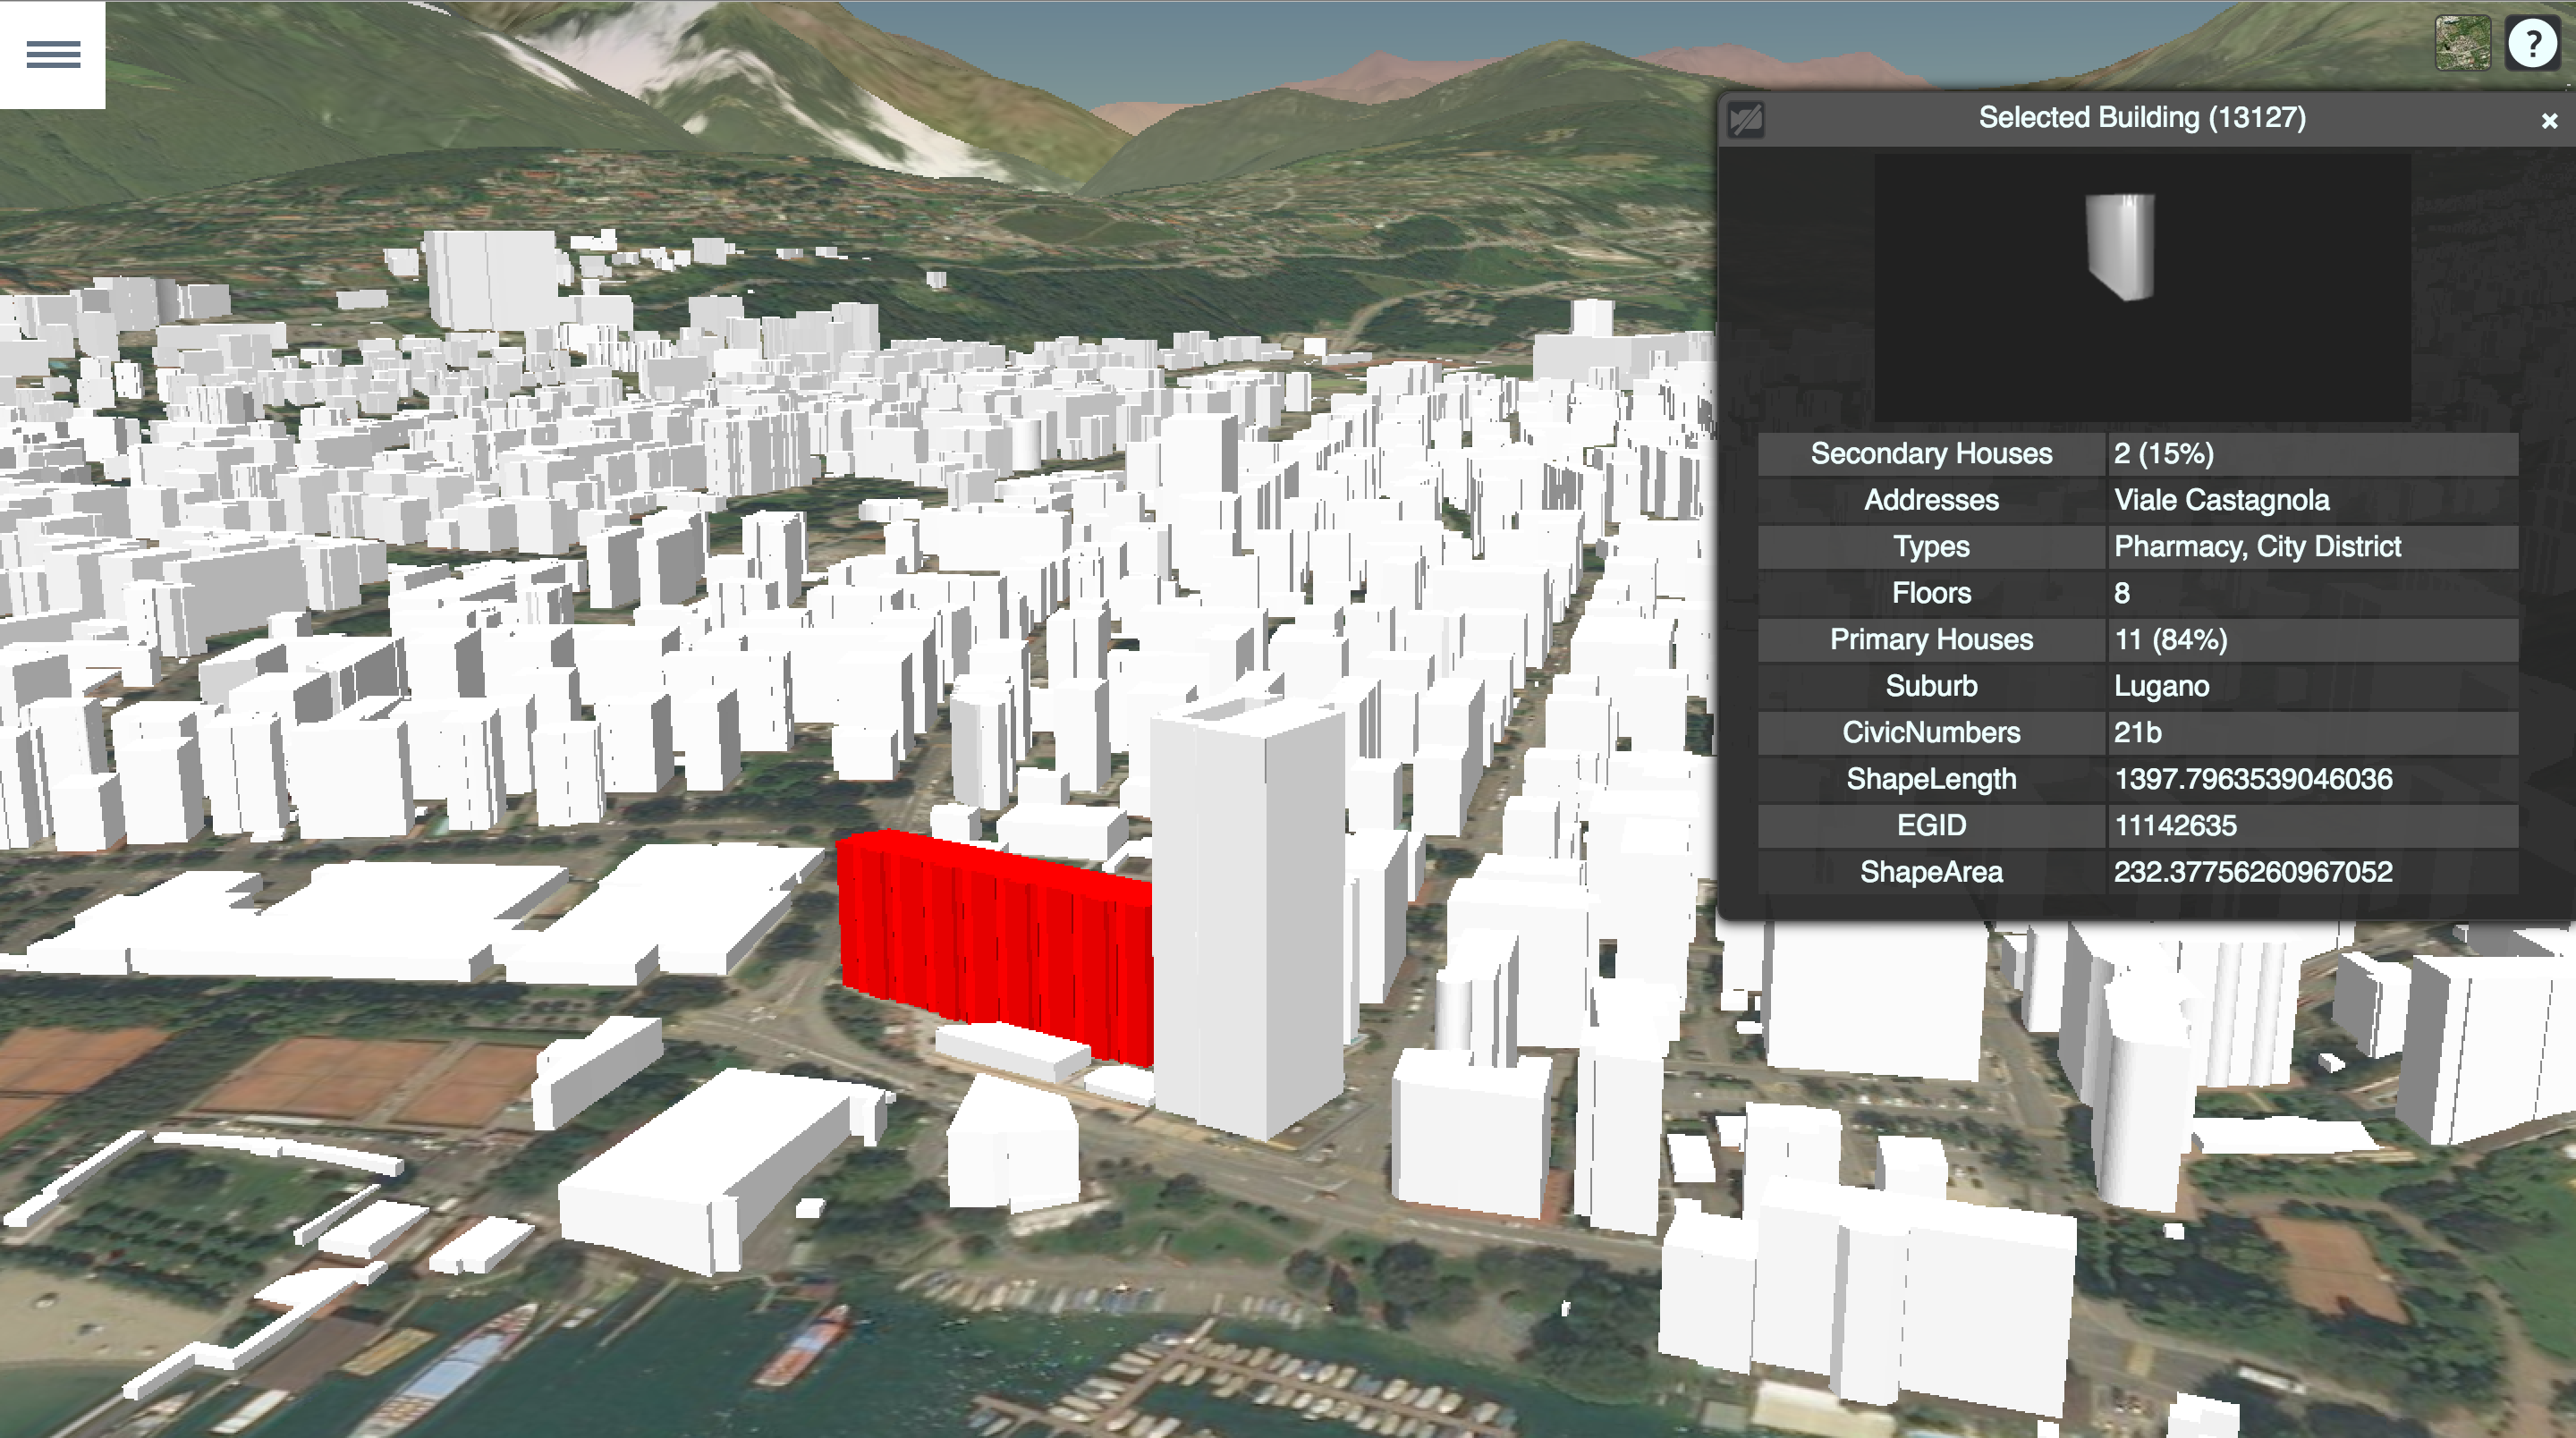
\includegraphics[width=0.8\textwidth]{chapter4/images/infoBox_city}
	\caption{Selecting a building will make the InfoBox appear automatically}
	\label{subfig:infoBox_city}
	\end{figure}
\begin{figure} [h]
	\centering
	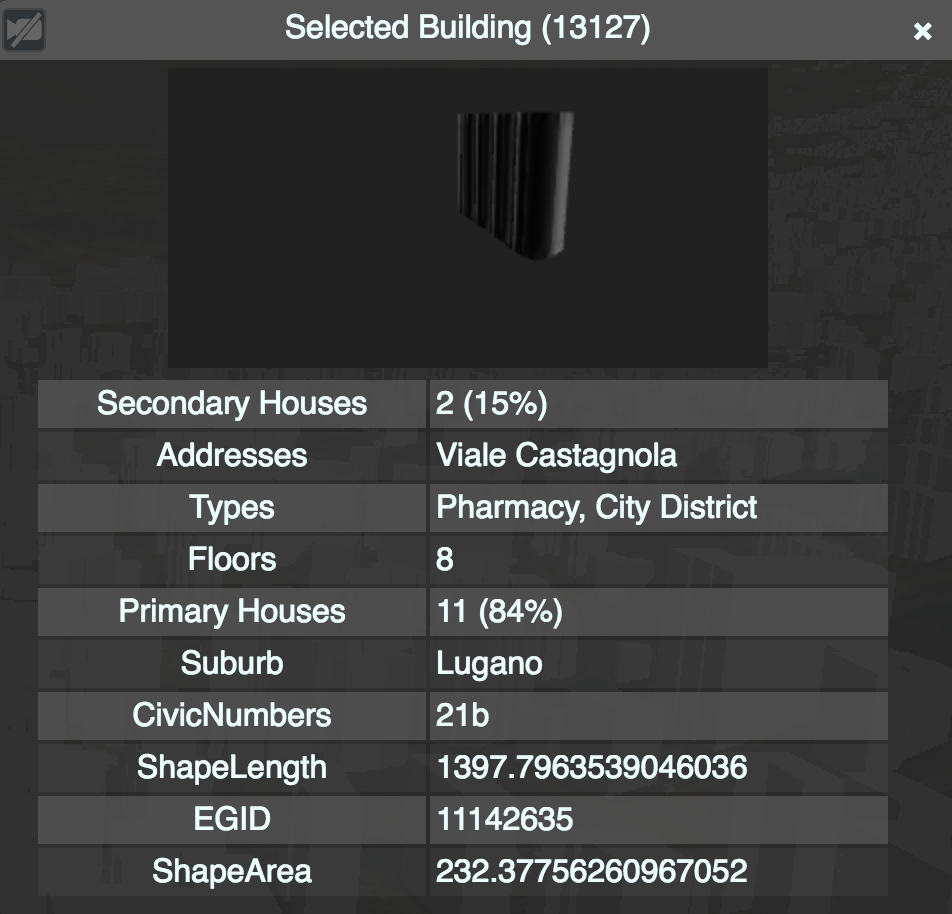
\includegraphics[width=0.5\textwidth]{chapter4/images/infoBox}
	\caption{A detailed look at the InfoBox}
	\label{subfig:infoBox}
\end{figure}
The first field displayed is a 3D representation of the model of the building clicked without its surrounding environment. It is possible to interact with this canvas in order to rotate and zoom the building model freely.\\
After, a list of useful information about the building follows: the length of this list changes from building to building depending on the availability of the information.\\
The building clicked in the example of figure \ref{fig:infoBox} presents all the possible available information that an user can get about a building.\\
The fields of the displayed data are denoted as follows: 
\begin{itemize}
\item {\bf Types} provides the list of groups in which the building is present. Groups are defined by the OpenStreetMap APIs and are used to represent the usage of the buildings which, conceptually, have characteristics in common. Examples of types are: Post Office, Pharmacy, Hospital, University etc \dots.
\item {\bf Floors} is the number of floors that the building possesses
\item {\bf Shape Length \& Shape Area} represent the size of buildings available for consultancy, they are measured in length and area both expressed in meters.
\item {\bf Street Name \& Civic Numbers} are the data concerning the addresses of the street where the building is located. There could be more than one street name and civic numbers in case the building has many of them (e.g., different entrances in the same building that are on different streets). Addresses data are taken from Swisstopo APIs and, if not available from this service, OpenStreetMap APIs are used.
\item {\bf EGID} the unique identifier of the building given by the Swiss REA 
\item {\bf Suburb} represents the suburb in which the building is located
\item {\bf Primary \& Secondary houses} represents both the number of primary and secondary houses in the selected building and the percentage that each value represents over the total number of houses in that building
\end{itemize}

\subsection{Visualize the City}
The first tab available to the user when the side--bar is opened, is the Visualize Tab. It is divided into three main subsections: ``Show on the map'', ``Color city'' and ``Show Suburbs''.\\

The first subsection contains two checkboxes: the first one, let the user show the geolocalization, i.e., the position of the device from which the user is using \applicationName. The second checkbox, if checked, shows the position of webcams located around Lugano; this webcams continuously stream videos of the city. In Figure \ref{fig:mapPins} it is possible to see the result on the map, when both checkboxes are checked.
\begin{figure} [H]
\centering
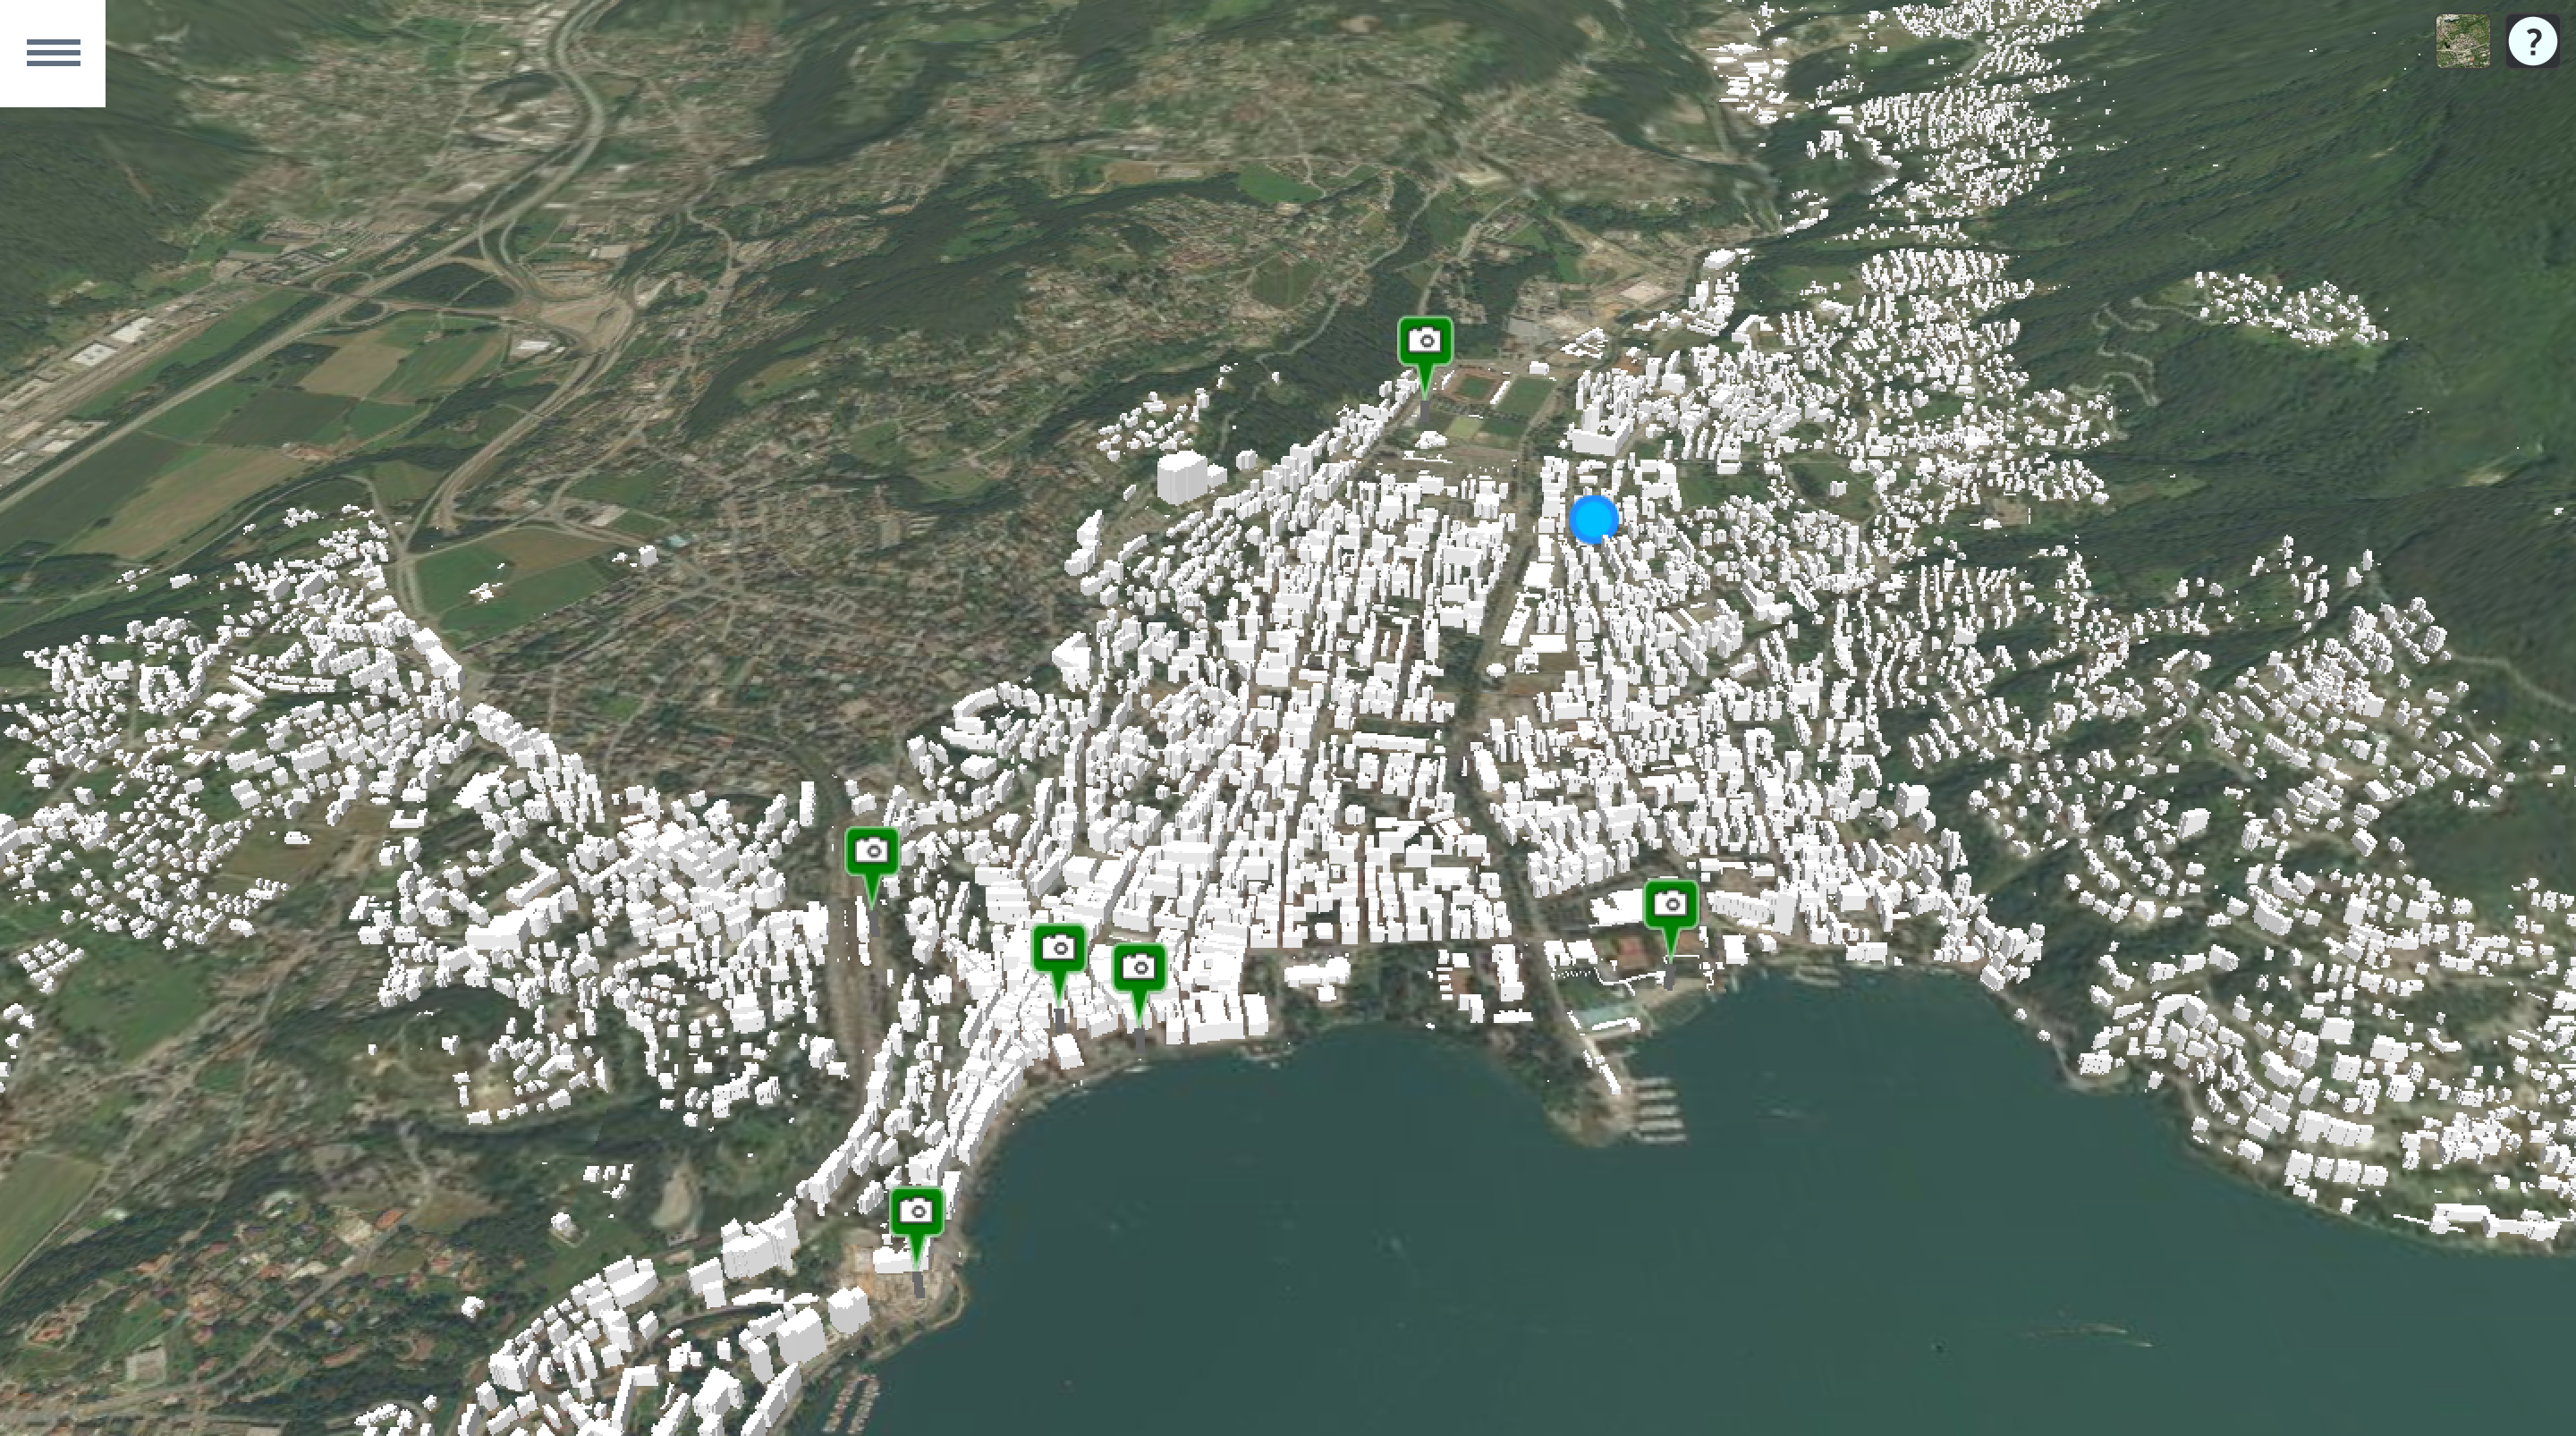
\includegraphics[width=.8\textwidth]{chapter4/images/mapPins}
\caption{When both checkboxes are checked, geolocalization and webCams positions are shown on the map}
\label{fig:mapPins}
\end{figure}
Since the 3D visualization had still to allow the user to exactly locate the position of these pins, whenever the visualization is more zoomed it it, a ``stick'' is created starting from the ground and ending at the bottom of the pin, as it is shown in Figure \ref{fig:3dPins}.\\

\begin{figure} [H]
\centering
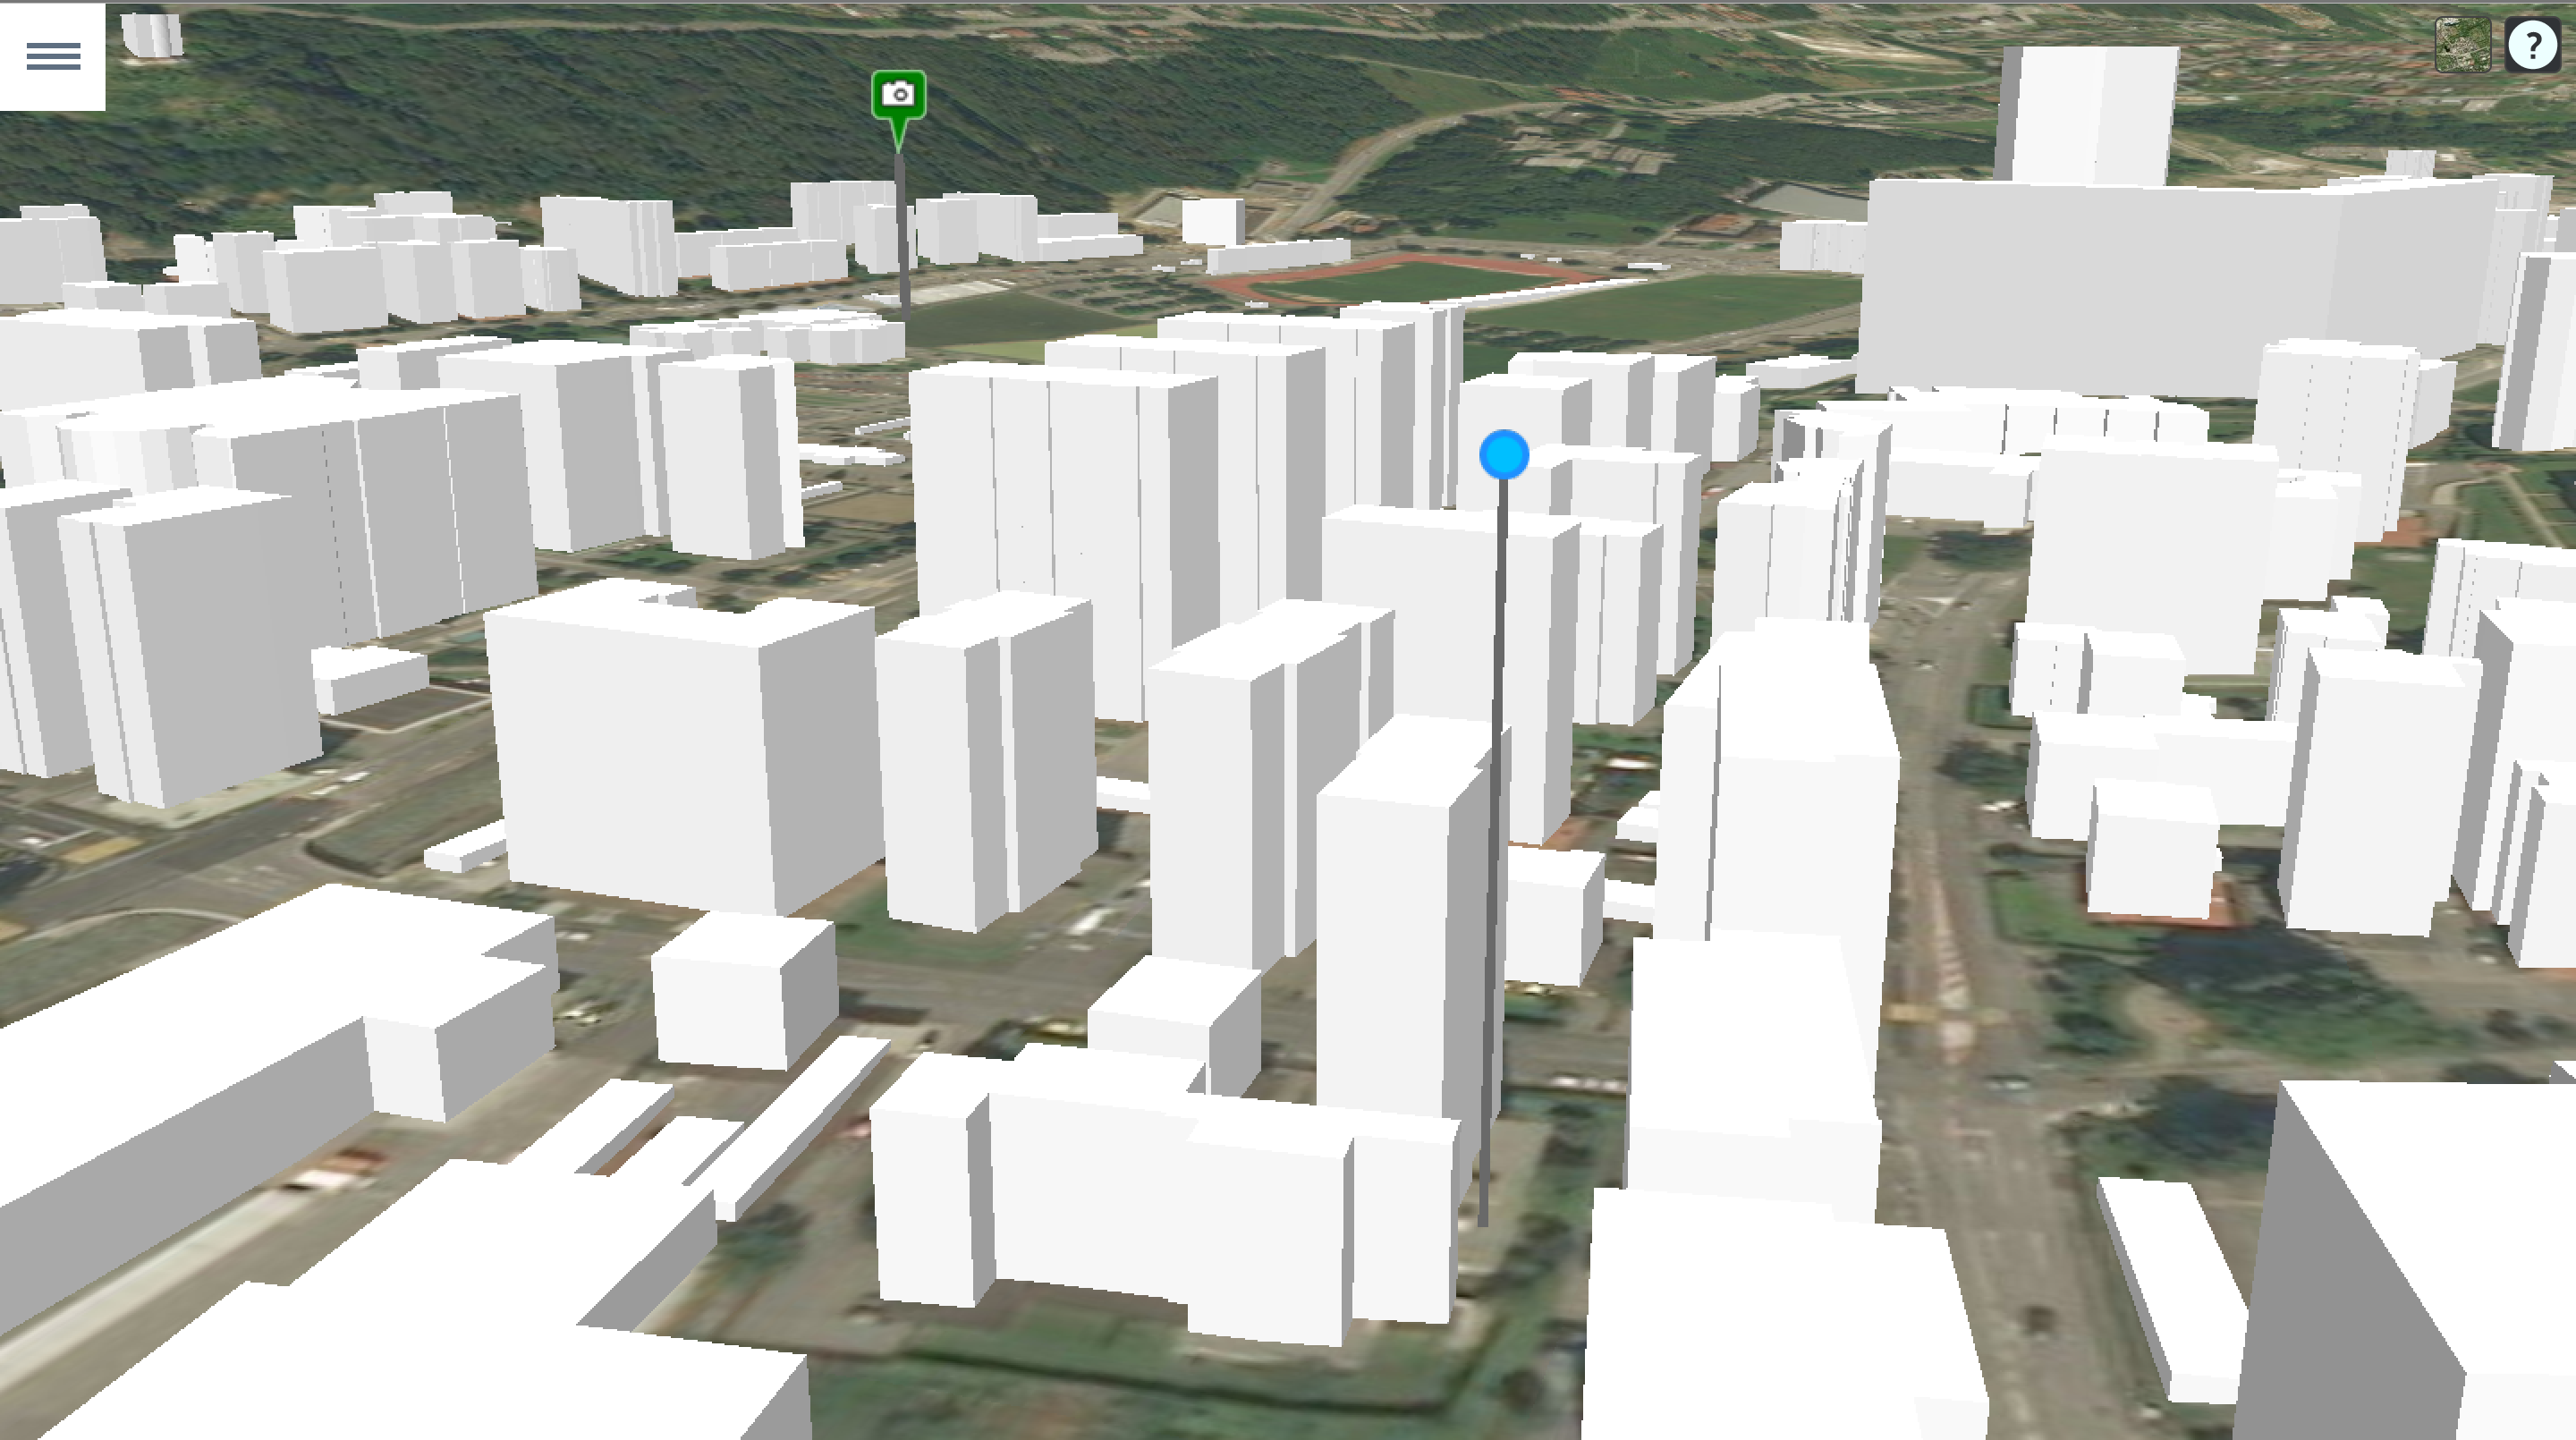
\includegraphics[width=.8\textwidth]{chapter4/images/3dPins}
\caption{The ``Stick'' that connects the ground to the pins}
\label{fig:3dPins}
\end{figure}
In the second subsection three radio buttons can be found: the first one is used to reset the color of the entire city to the default color. The second colours the buildings in the city based on their height (Figure\ref{fig:application_byHeight}). The third one is used to colour the entire city based on its suburbs and so every suburb has a different color(Figure \ref{fig:application_showSuburb} ).\\

\begin{figure} [H]
\centering
\includegraphics[width=.8\textwidth]{chapter4/images/application_bySuburb}
\caption{A Visualization of the city of Lugano where every suburb is coloured differentrly}
\label{fig:application_bySuburb}
\end{figure}
\begin{figure} [H]
\centering
\includegraphics[width=.8\textwidth]{chapter4/images/application_byHeight}
\caption{A Visualization of the city of Lugano where every building is colorued based on its height}
\label{fig:application_byHeight}
\end{figure}
The third and last subsection, contains the list of checkboxes representing all the suburbs in the city and their respective colours. By default all checkboxes are checked but uncheck them will result in hiding the desired suburb as show in Figure \ref{fig:application_showSuburb}.
\begin{figure} [H]
\centering
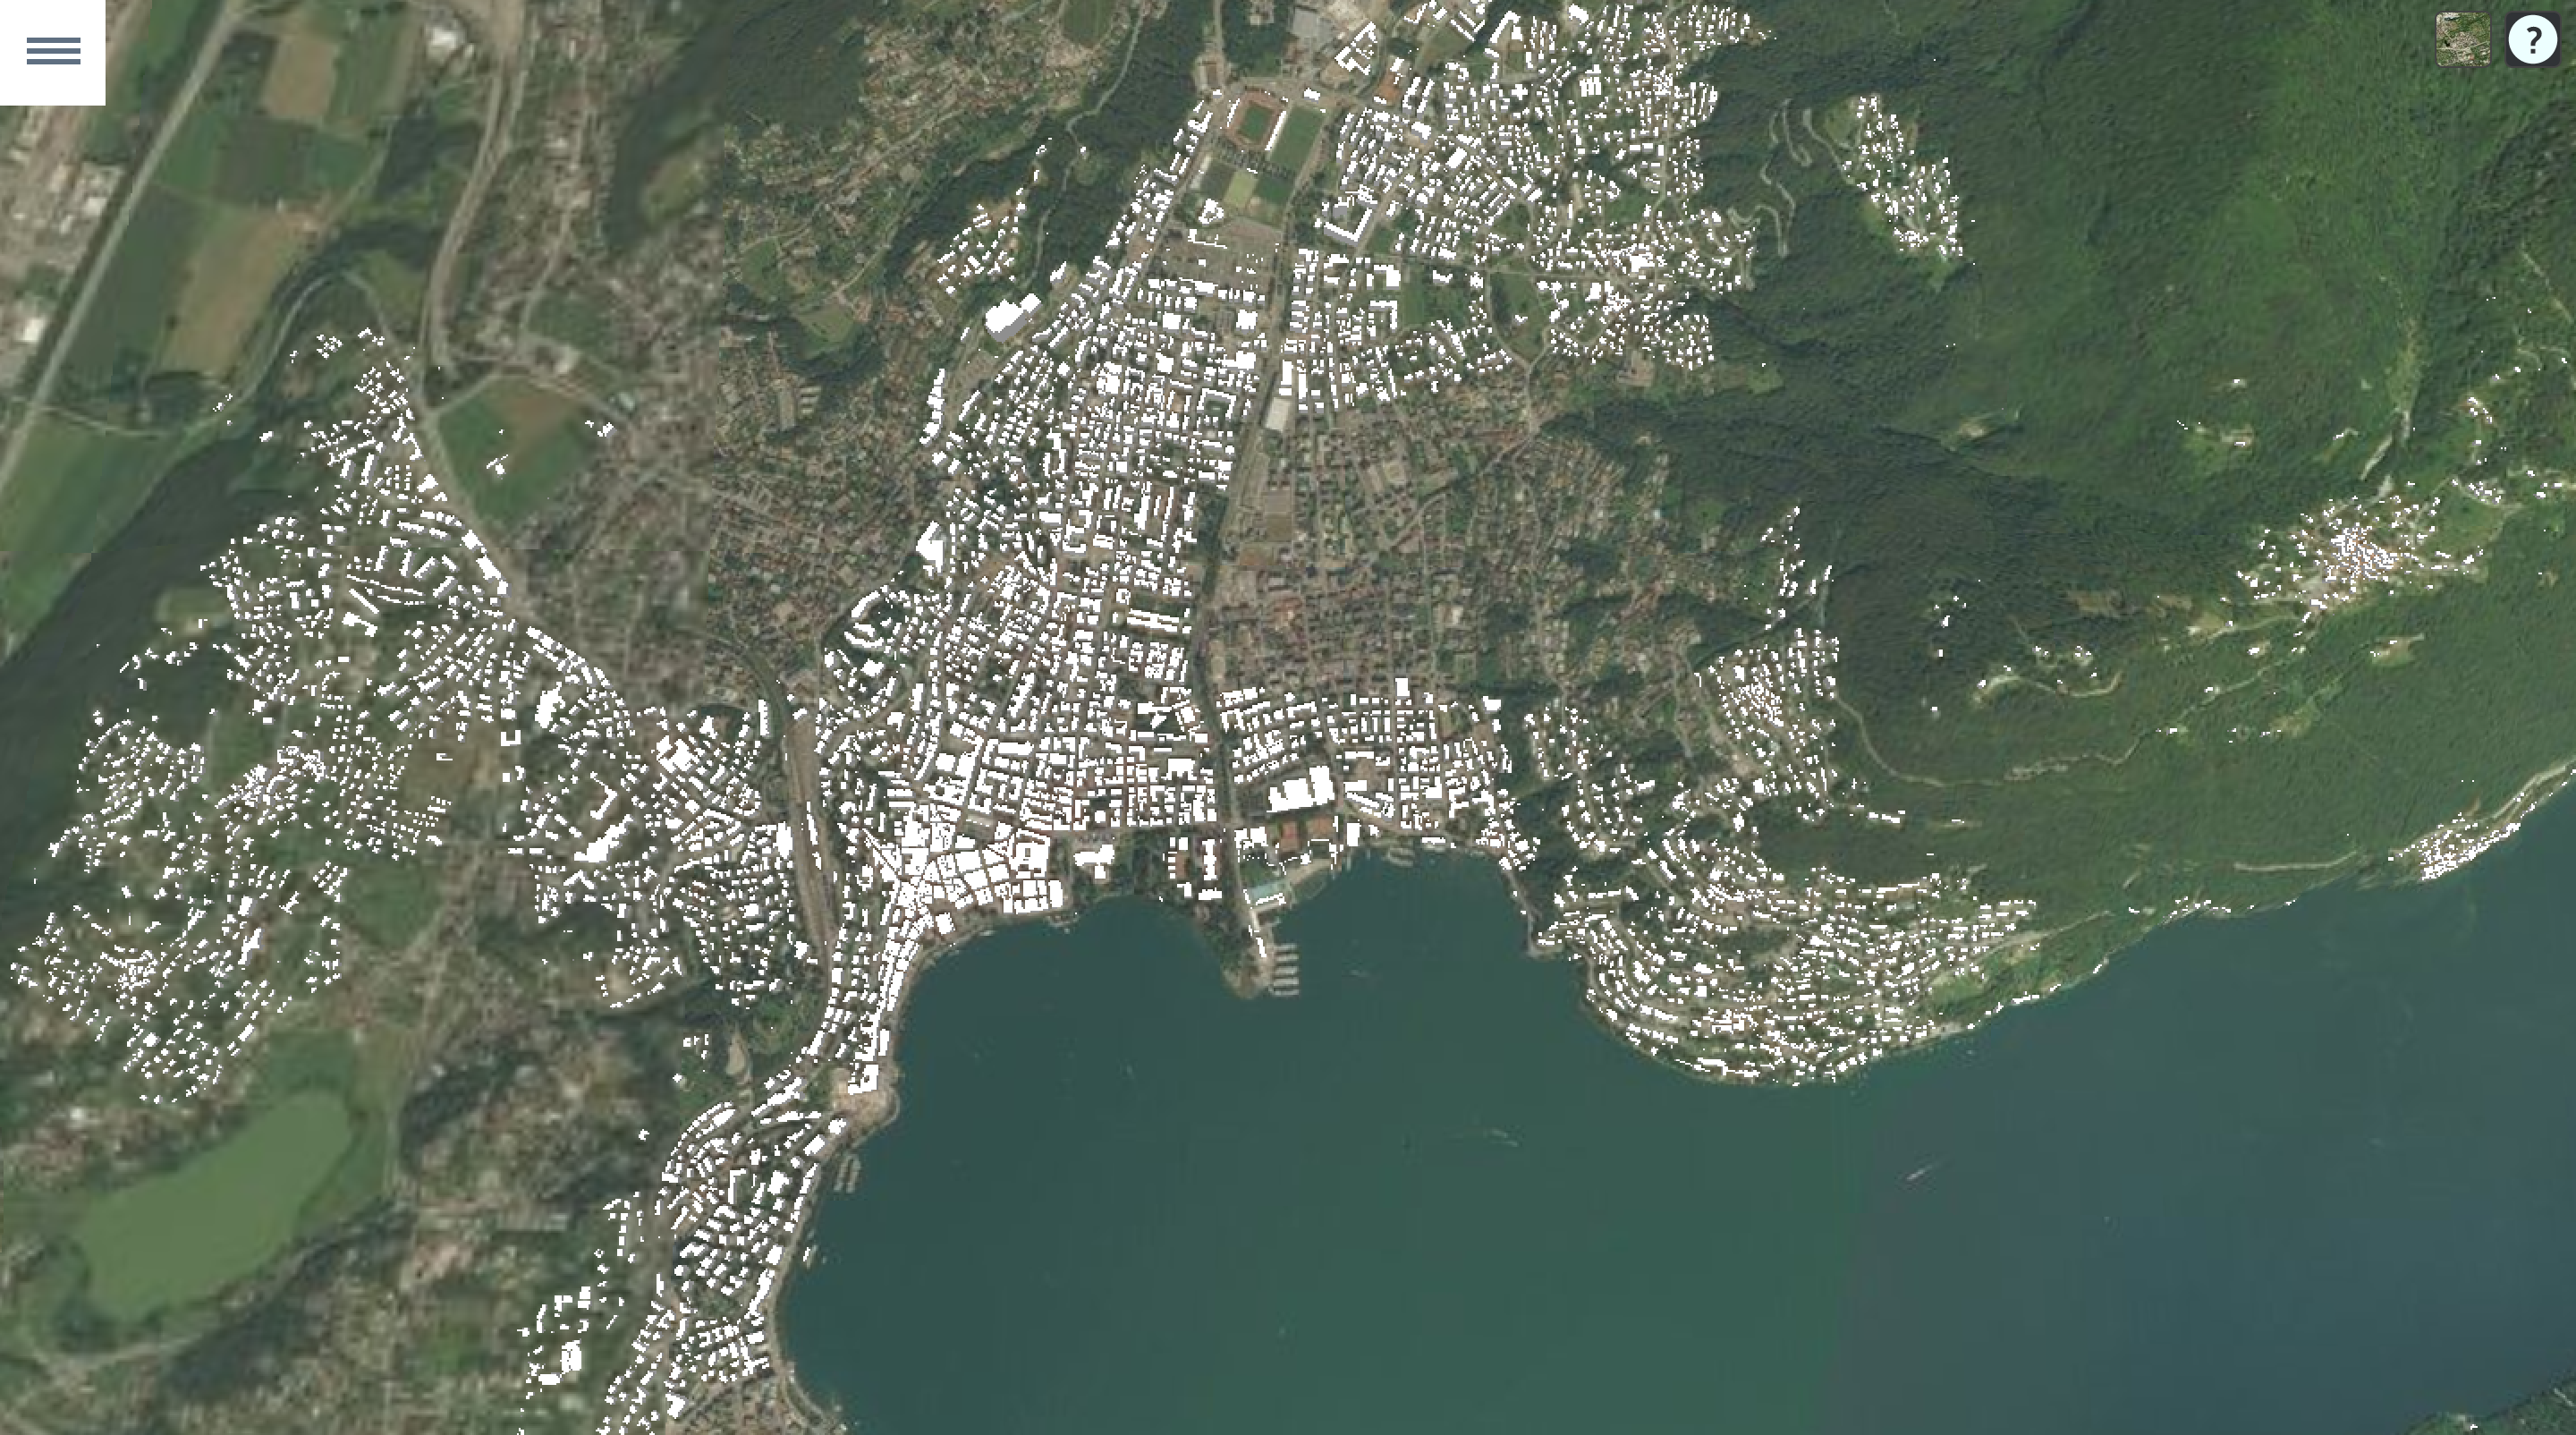
\includegraphics[width=.8\textwidth]{chapter4/images/application_showSuburb}
\caption{A Visualization of the city of Lugano where the suburb Viganello is hidden}
\label{fig:application_showSuburb}
\end{figure}

\subsection{The Query System}
\subsubsection{Building Selection}
The following use cases show what actions can be performed using the visual query system. The interactions proposed are accessible through the apposite ``Query City'' selection tab in the provided sidebar.\\
As it is possible to see on Figure \ref{fig:query_city_tab} in the previous chapter, \applicationName\ allows the user to perform from very single to more complex query on the entire city. Some examples are shown in the following images:
\begin{figure} [H]
\centering
\includegraphics[width=.8\textwidth]{chapter4/images/query1}
\caption{Result of the query: ``Get all the banks in Lugano''}
\label{fig:query1}
\end{figure} 
\begin{figure} [H]
\centering
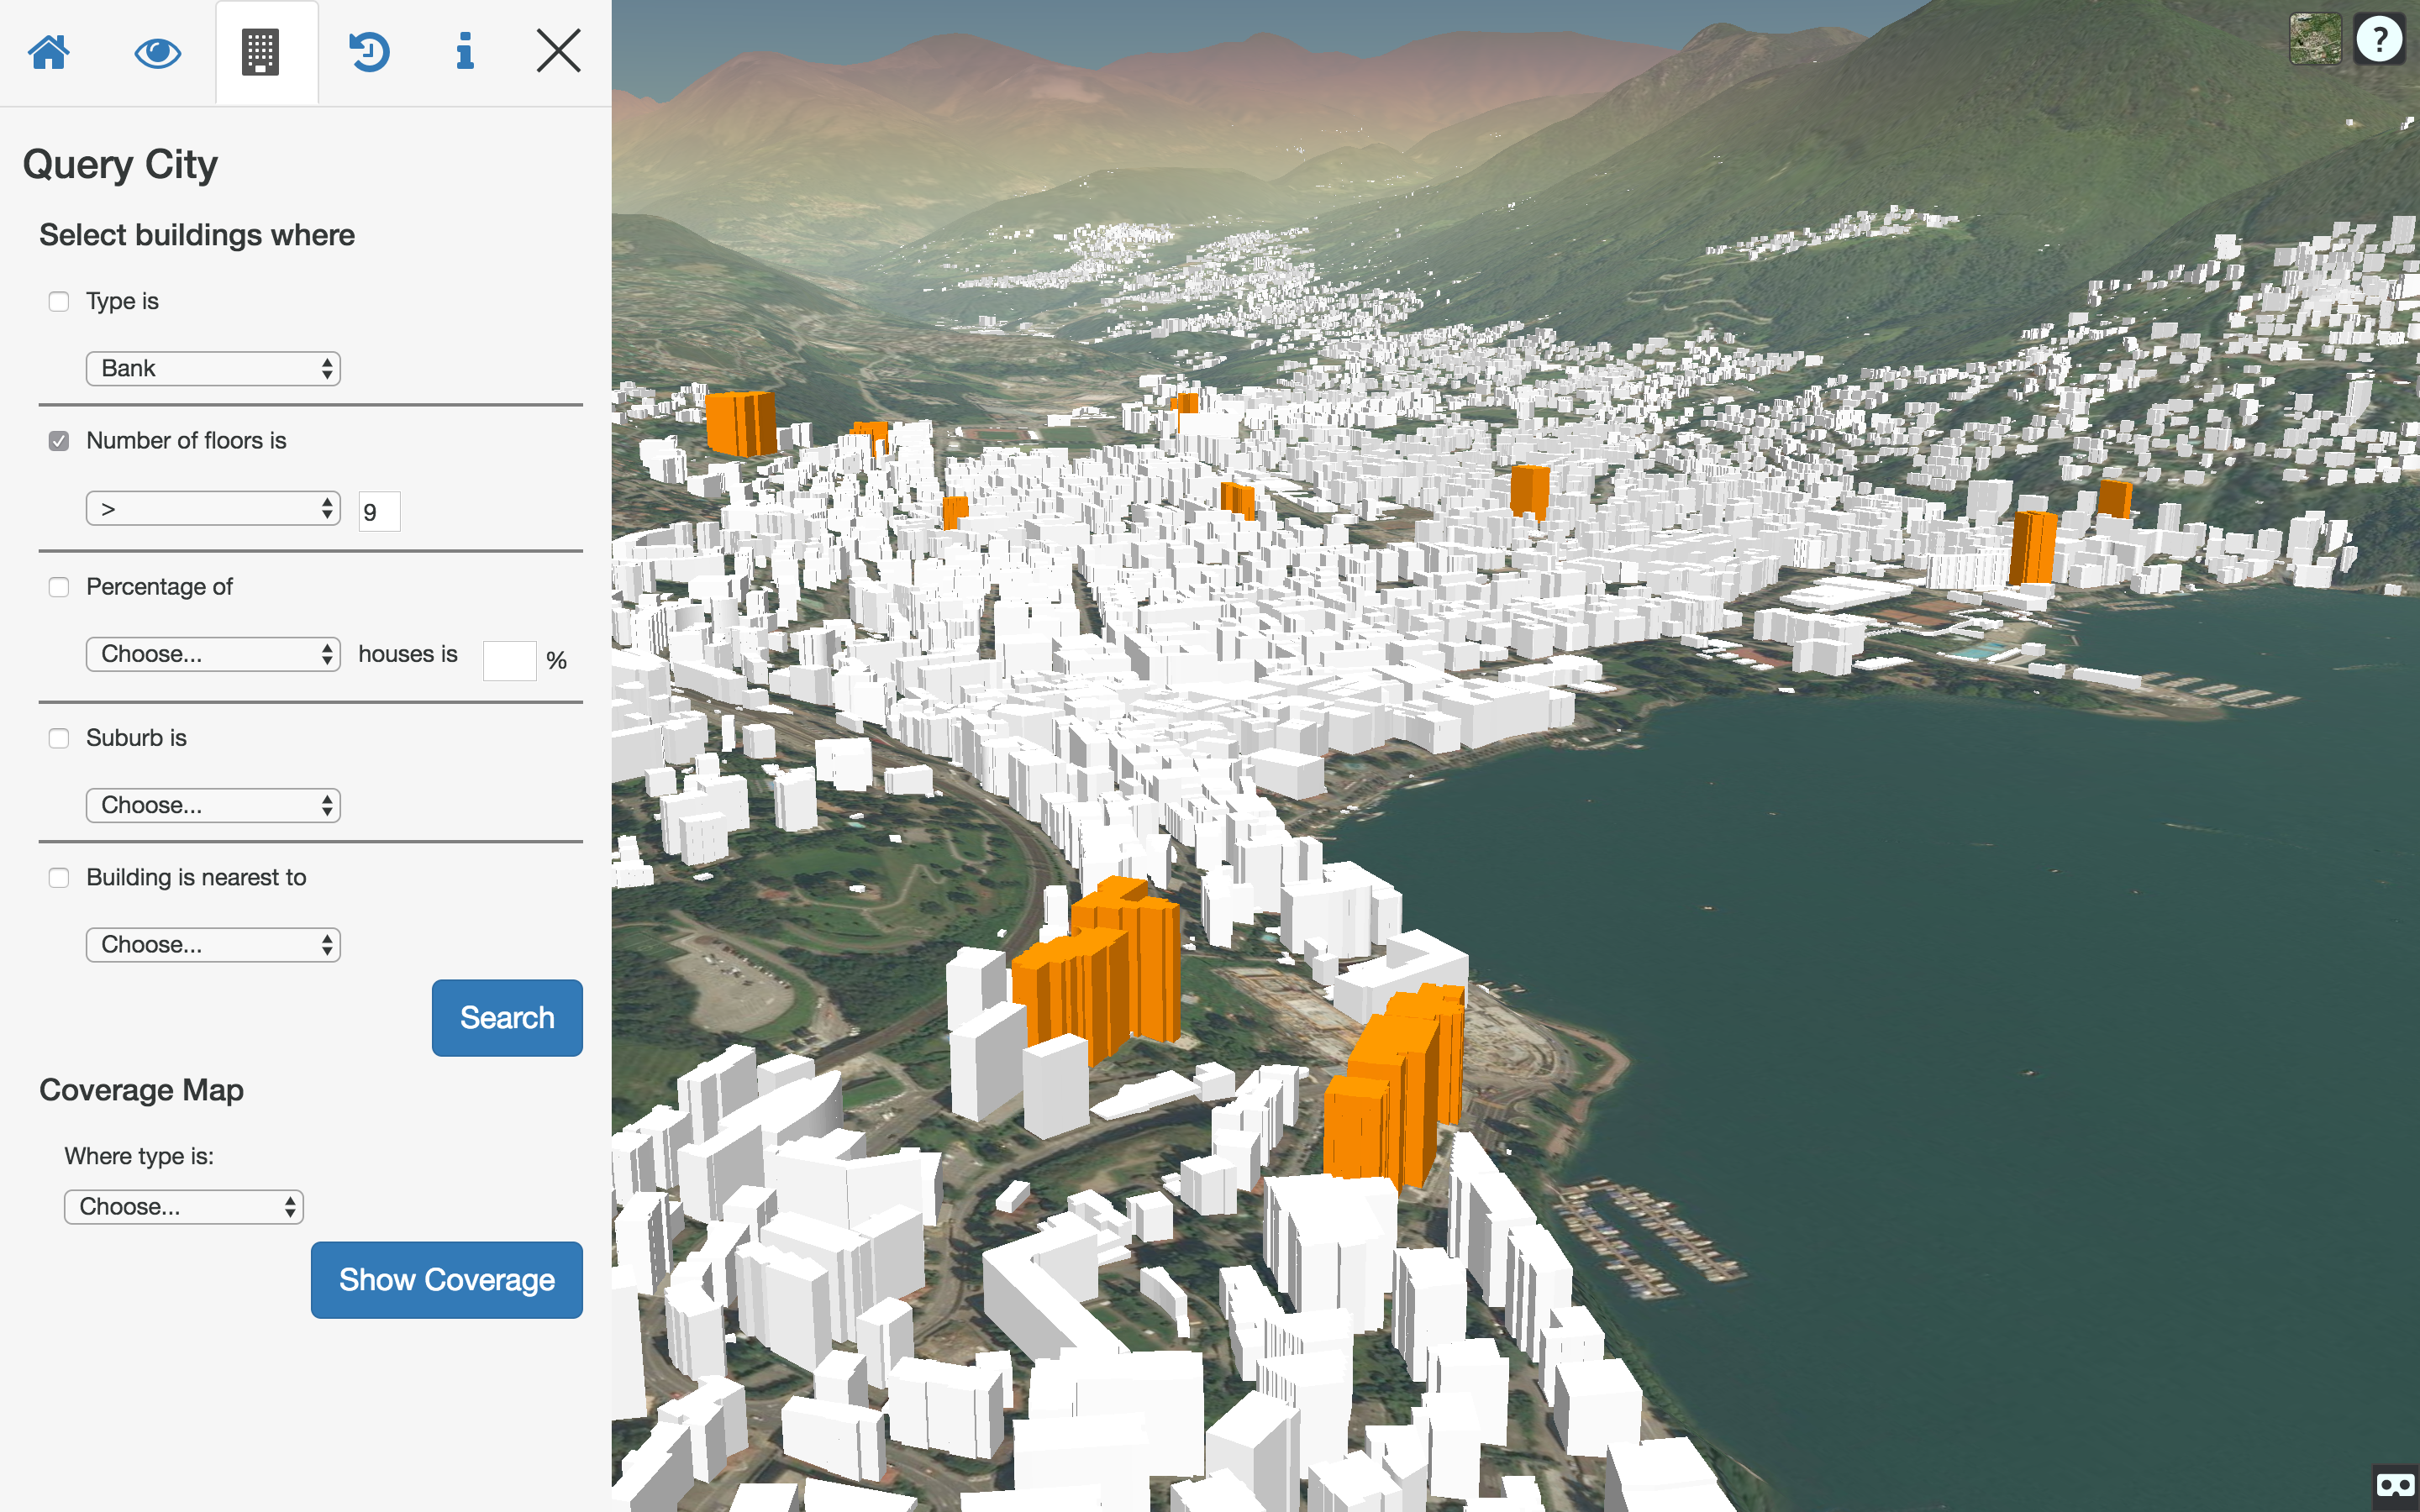
\includegraphics[width=.8\textwidth]{chapter4/images/query2}
\caption{Result of the query: ``Get all the buildings with more than 9 floors in Lugano''}
\label{fig:query2}
\end{figure} 
\begin{figure} [H]
\centering
\includegraphics[width=.8\textwidth]{chapter4/images/query3}
\caption{Result of the query: ``Get all the hospitals in Viganello (Suburb of Lugano)''}
\label{fig:query3}
\end{figure} 
\begin{figure} [H]
\centering
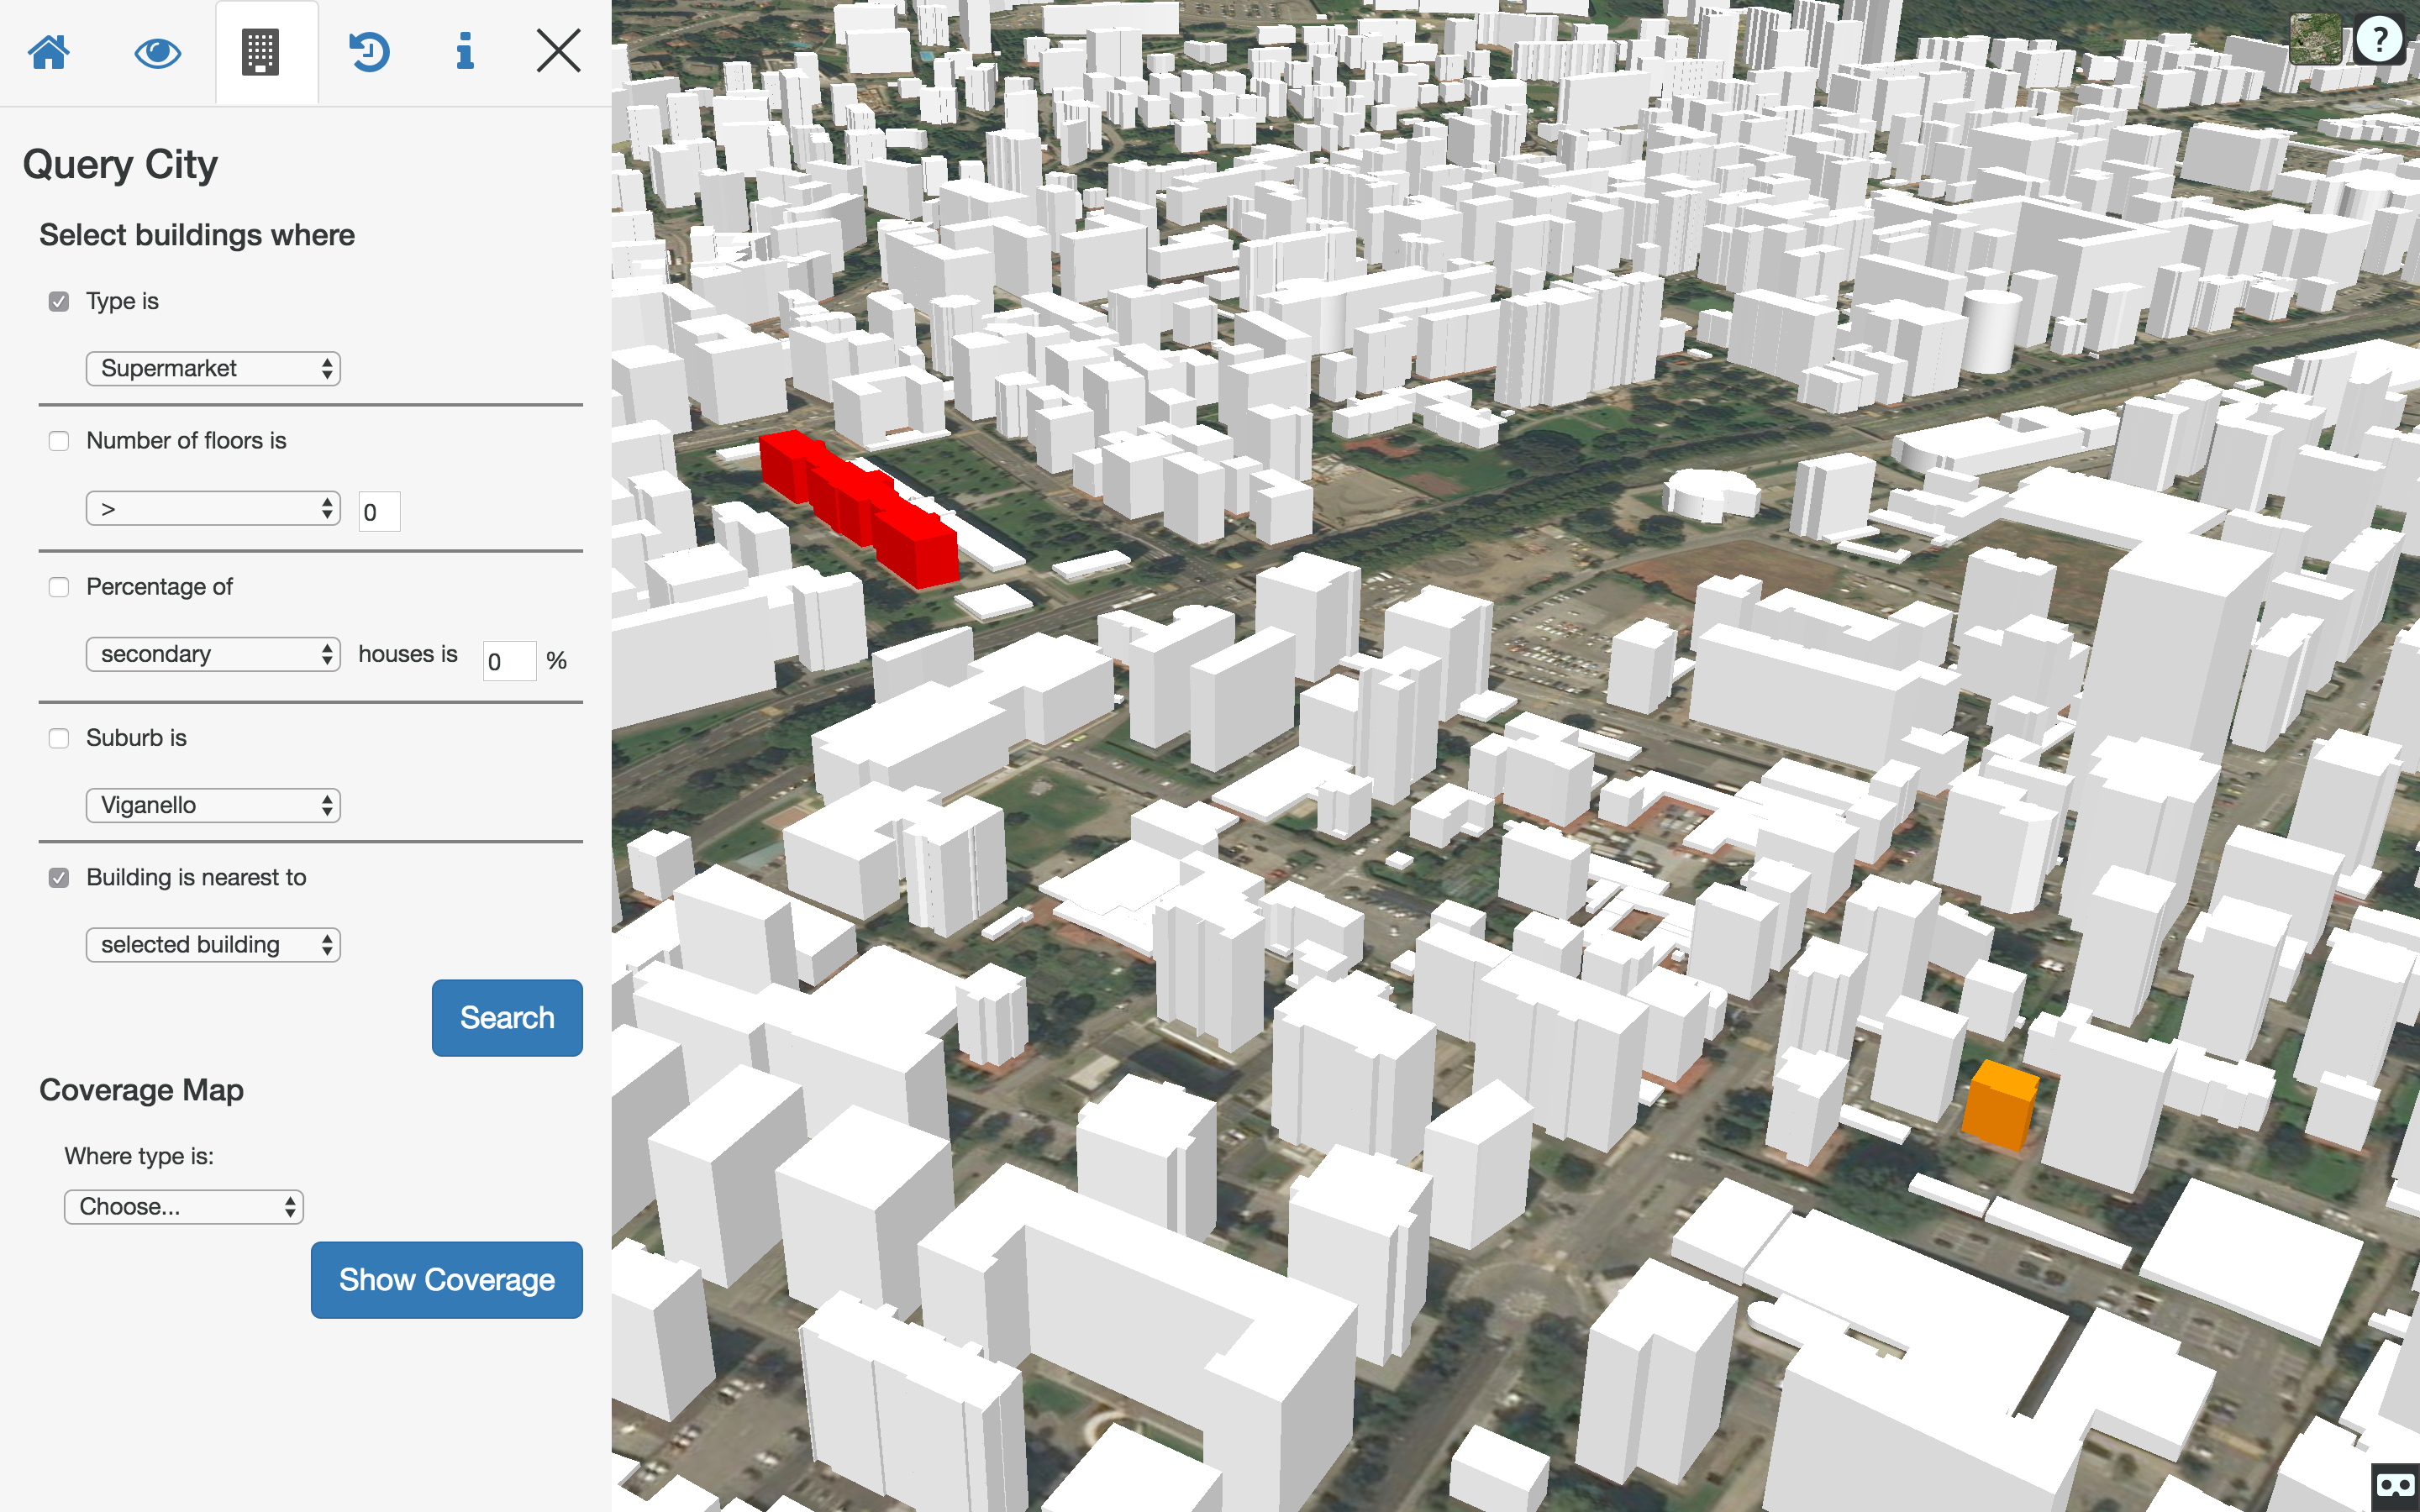
\includegraphics[width=.8\textwidth]{chapter4/images/query4}
\caption{Result of the query: ``Get nearest Supermarket near the selected building''}
\label{fig:query4}
\end{figure} 
\begin{figure} [H]
\centering
\includegraphics[width=.8\textwidth]{chapter4/images/query5}
\caption{Result of the query: ``Get all the buildings with less than 10 floors and where the percentage of primary houses is up to $70\%$ in the Suburb of Lugano''}
\label{fig:query5}
\end{figure} 

\subsubsection{City Gradient Map}
\applicationName\ also allows to visualize the coverage of a specific type--building with respect to the entire city. The coverage is grafically shown coloring the buildings differently depending on their distance from a hotspot.\\

In particular, whenever a user does a coverage query, the hotspot or hotspots (in the case of multiple buildings of the same type) will be colored in red. The other buildings will be colored using an interpolation from ``Lime green'' (i.e., nearest buildings to the hotspost) to white (i.e., farthest buildings to the hotspot). 
If a building is inside the coverage area of two hotspot, let us say hotspot$_{1}$ and hotspot$_{2}$, its color will be determined by the mean between the distance of the building from hotspot$_{1}$ and the distance of the building from hotspot$_{2}$.\\

Figures \ref{fig:query6} and \ref{fig:query7} show two examples of coverage of particular hotspot in the city of Lugano. The former represents the coverage of banks, the latter the coverage of hospitals in the city.
\begin{figure} [H]
\centering
\includegraphics[width=.8\textwidth]{chapter4/images/query6}
\caption{Coverage map of banks in the city of Lugano}
\label{fig:query6}
\end{figure} 
\begin{figure} [H]
\centering
\includegraphics[width=.8\textwidth]{chapter4/images/query7}
\caption{Coverage map of hospitals in the city of Lugano}
\label{fig:query7}
\end{figure} 